\section*{ÔN TẬP KIỂM TRA CUỐI KÌ 1 - ĐỀ 04}
\setcounter{ex}{0}\setcounter{bt}{0}
\Opensolutionfile{ans}[ans/ansBTTeX4]

\noindent\textbf{I. PHẦN TRẮC NGHIỆM:}
\begin{ex}%[1H4H4-2]
\immini{Cho hình chóp $S. ABCD$. Gọi $M$, $N$, $P$ lần lượt là trung điểm các cạnh $SA$, $AB$ và $AD$ (tham khảo hình bên).
Mặt phẳng $\left(MNP\right)$ song song với mặt phẳng nào dưới đây?
\choice
{\True $\left(SBD\right)$}
{$\left(SCD\right)$}
{$\left(ABCD\right)$}
{$\left(SBC\right)$}}
{
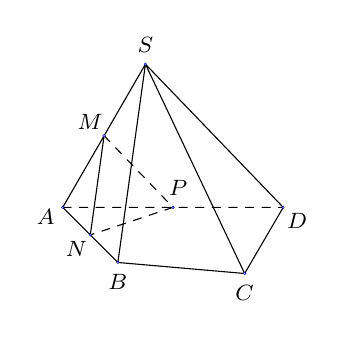
\begin{tikzpicture}[xscale=0.7,yscale=0.7,>=stealth, font=\footnotesize, line join=round, line cap=round,declare function={h=3;}]
\path
(0,0) coordinate (A)
(1,-1) coordinate (B)
(3.3,-1.2) coordinate (C)
(4,0) coordinate (D)
(A)+(60:h) coordinate (S)
(barycentric cs:A=1,S=1)coordinate(M)
(barycentric cs:A=1,B=1)coordinate(N)
(barycentric cs:A=1,D=1)coordinate(P)
;
\draw[dashed] (M)--(P)--(N) (A)--(D);
\draw (C)--(S)--(A)--(B)--(C)--(D)--(S)--(B) (M)--(N);
\foreach \p/\g in{A/-150,B/-90,C/-90,D/-45,S/90,M/135,N/-135,P/75}
\shade[shading=ball](\p)circle(.03)node[shift={(\g:.25)},scale=1]{$\p$};
\end{tikzpicture}
}
\loigiai{
Ta có $MP\parallel SD;MP\not\subset\left(SBD\right)$ $\Rightarrow$ $MP\parallel \left(SBD\right)$.\\
$MN\parallel SB;MN\not\subset\left(SBD\right)$ $\Rightarrow$ $MN\parallel \left(SBD\right)$\\
$MN$ cắt $MP$ trong $\left(MNP\right)$\\
Từ đó suy ra $\left(MNP\right)\parallel \left(SBD\right)$.
}
\end{ex}

\begin{ex}%[1H4H1-3]%[Dự án đề ôn tập Toán Khối 11 HK1 NH23-24-Dot 1-Vương Quốc Phong]%[CTST - Đề số 3]
Cho hình chóp $S.ABCD$ có đáy là hình thang $ABCD$ ($AB \cap CD = O$). Khẳng định nào sau đây \textbf{sai}?
\choice
{Hình chóp $S.ABCD$ có $4$ mặt bên}
{Giao tuyến của hai mặt phẳng $(SAC)$ và $(SBD)$ là $SO$}
{Giao tuyến của hai mặt phẳng $(SAD)$ và $(SBC)$ là $SI$ ($I$ là giao điểm của $AD$ và $BC$)}
{\True Giao tuyến của hai mặt phẳng $(SAB)$ và $(SAD)$ là đường trung bình của $ABCD$}
\loigiai{
Ta có $(SAB) \cap (SAD) = SA$ và $SA$ không thể là đường trung bình của hình thang $ABCD$.
}
\end{ex}

\begin{ex} %[1D3H2-2]
${\mathop{\lim}\limits_{x\to-2}} \left(2x^2+1\right)$ bằng

\choice{\True $9$}
{$5$}
{$-7$}
{$+\infty$}
\loigiai{
Ta có ${\mathop{\lim}\limits_{x\to-2}} \left(2x^2+1\right)=2\left(-2\right)^2+1=9$.
}
\end{ex}

\begin{ex}%[1D2H3-3]
Cho cấp số nhân $2,4,8,\ldots$ Số hạng tổng quát của cấp số nhân đã cho là
\choice
{$u_{n}=2^{n+1}$}
{$u_{n}=4^{n}$}
{\True $u_{n}=2^{n}$}
{$u_{n}=2^{n-1}$}
\loigiai{
Số hạng tổng quát của CSN: $u_{n}=u_{1} \cdot q^{n-1}=2 \cdot 2^{n-1}=2^{n}$.
}
\end{ex}

\begin{ex}%[1D3N3-1]
Hàm số nào sau đây liên tục trên $\mathbb{R}$?
\choice
{\True $y=\sqrt{x^2+2023}$}
{$y=\dfrac{1}{x+2023}$}
{$y=\tan x$}
{$y=\sqrt{x-1}$}
\loigiai{
Hàm số $y=\sqrt{x^2+2023}$ có tập xác định là $\mathbb{R}$ nên nó liên tục trên $\mathbb{R}$.
}
\end{ex}

\begin{ex}Cau20%[1H4N3-1]
Trong không gian có bao nhiêu vị trí tương đối giữa đường thẳng và mặt phẳng?
\choice
{$1$}
{$2$}
{\True $3$}
{$4$}
\loigiai{
Có ba vị trí tương đối giữa đường thẳng và mặt phẳng.
}
\end{ex}

\begin{ex}%[1H4N1-3]%[Lê Xuân Hòa ]
Cho $4$ điểm $A$, $B$, $C$, $D$ không cùng nằm trên mặt phẳng. Trên $AB$, $AD$ lần lượt lấy $2$ điểm $M$, $N$ sao cho $MN$ cắt $BD$ tại $I$. Điểm $I$ không thuộc mặt phẳng nào sau đây?
\choice
{$(ABD)$}
{$(BCD)$}
{$(CMN)$}
{\True $(ACD)$}
\loigiai{
\immini{Vì $I=MN\cap BD$ nên $I\in\left(ABD\right)$, $I\in\left( BCD\right)$, $I\in\left(CMN\right)$.
}
{
\begin{tikzpicture}[line join=round, line cap=round,thick,scale=0.6]
\coordinate (A) at (0,4);
\coordinate (D) at (-4,0);
\coordinate (B) at (0,-2);
\coordinate (C) at (3,0);
\coordinate (M) at  ($(A)!0.3!(B)$);
\coordinate (N) at  ($(A)!0.6!(D)$);
\tkzInterLL(B,D)(M,N)
\tkzGetPoint{I}
\draw(A)--(D) (A)--(B) (A)--(C) (B)--(C) (D)--(B) (M)--(I) (D)--(I);
\draw[dashed,thin](D)--(C);
\tkzLabelPoints[left](I)
\tkzLabelPoints[above left](N)
\tkzLabelPoints[right](M, C)
\tkzLabelPoints[above](A)
\tkzLabelPoints[below](B,D)
\end{tikzpicture}
}
}
\end{ex}

\begin{ex}%[1D1H4-6]
Tập giá trị của hàm số $y=5\sin x-12\cos x$ là
\choice
{$[-12;5]$}
{\True $[-13;13]$}
{$[-17;17]$}
{$(-13;13)$}
\loigiai{
Ta có
\allowdisplaybreaks
\begin{eqnarray*}
y &=& 5\sin x-12\cos x=13\left(\dfrac{5\sin x-12\cos x}{13}\right)\\
&=& 13\left( \sin \alpha\sin x-\cos \alpha \cos x\right)\\
&=& -13\cos (x+\alpha).\quad \left(\text{với}\, \sin\alpha=\dfrac{5}{13},\cos \alpha=\dfrac{12}{13}\right)
\end{eqnarray*}
Lại có $-1\le \cos (x+\alpha)\le 1\Leftrightarrow -13\le -13\cos (x+\alpha)\le 13$.\\
Vậy tập giá trị hàm số $y=5\sin x-12\cos x$ là $[-13;13]$.
}
\end{ex}

\begin{ex}%[Pj10-1-HK1-NH23-24(CD)--TeamTeXHoa--Võ Thị Thùy Trang]%[1D1H4-3]
Hàm số $y=\sin x$ đồng biến trên khoảng nào dưới đây?
\choice
{$\left(-\pi;\dfrac{\pi}{2}\right)$}
{\True $\left(-\dfrac{\pi}{2};0\right)$}
{$\left(0;\pi \right)$}
{$\left(\dfrac{\pi}{2};\pi \right)$}
\loigiai{
Dựa vào đồ thị hàm số $y=\sin x$ ta thấy đồ thị hướng đi lên từ trái sang phải trên $\left(-\dfrac{\pi}{2};0\right)$.\\
Nên hàm số đồng biến trên khoảng $\left(-\dfrac{\pi}{2};0\right)$.  }
\end{ex}

\begin{ex}%[1D3H1-2]
Giới hạn $\lim\dfrac{3n-7}{2n^2+3n-1}$ bằng
\choice
{$\dfrac{3}{2}$}
{$3$}
{\True $0$}
{$\dfrac{-3}{2}$}
\loigiai{Ta có $\lim\dfrac{3n-7}{2n^2+3n-1}=\lim\left(\dfrac{1}{n}\cdot\dfrac{3-\dfrac{7}{n}}{2+\dfrac{3}{n}-\dfrac{1}{n^2}}\right)=0$.}
\end{ex}

\begin{ex}%[1D5H1-4]%[Dự án đề kiểm tra Toán 11 HKI NH23-24-Đợt 1- Phạm Phương]%[CTST-Đề số 5]
%[TH]
Doanh thu bán hàng trong 20 ngày được lựa chọn ngẫu nhiên của một cửa hàng được ghi lại ở bảng sau (đơn vị: triệu đồng):
\begin{center}
\begin{tabular}{|c|c|c|c|c|c|}
\hline
Doanh thu& $[5;7)$ & $[7;9)$ & $[9;11)$ & $[11;13)$ & $[13;15)$ \\
\hline
Số ngày&$2$ &$7$ &$7$ &$3$ &$1$ \\
\hline
\end{tabular}
\end{center}
Tìm mốt của mẫu số liệu ghép nhóm trên.
\choice
{$M_o=10{,}6$}
{$M_o=11{,}6$}
{\True $M_o=9$}
{$M_o=10$}
\loigiai{
Nhóm chứa mốt của mẫu số liệu trên là nhóm $[7;9)$ hoặc $[9;11)$.
\begin{enumerate}
\item [{\bf TH1.}] Xét nhóm $[7;9)$ ta có $u_m=7$, $u_{m+1}=9$, $n_m=7$, $n_{m+1}=7$, $n_{m-1}=2$.\\
Mốt của mẫu số liệu ghép nhóm là
\allowdisplaybreaks{\begin{eqnarray*}
M_o&=&u_m+\dfrac{n_m-n_{m-1}}{\left(n_m-n_{m-1}\right)+\left(n_m-n_{m+1}\right)}\cdot \left(u_{m+1}-u_m\right)\\
&=& 7+\dfrac{7-2}{\left(7-2\right)+\left(7-7\right)}\cdot \left(9-7\right)=9.
\end{eqnarray*} }
\item [{\bf TH2.}] Xét nhóm $[9;11)$ ta có $u_m=9$, $u_{m+1}=11$, $n_m=7$, $n_{m+1}=3$, $n_{m-1}=7$.\\
Mốt của mẫu số liệu ghép nhóm là
\allowdisplaybreaks{\begin{eqnarray*}
M_o&=&u_m+\dfrac{n_m-n_{m-1}}{\left(n_m-n_{m-1}\right)+\left(n_m-n_{m+1}\right)}\cdot \left(u_{m+1}-u_m\right)\\
&=& 9+\dfrac{7-7}{\left(7-7\right)+\left(7-3\right)}\cdot \left(11-9\right)=9.
\end{eqnarray*} }
\end{enumerate}
Vậy mốt của mẫu số liệu ghép nhóm trên là $M_o=9$.
}
\end{ex}

\begin{ex}%[1D1N4-2]%[Dự án đề ôn tập Toán khối 11 HKI NH23-24-Dot 1-Xuan Vy Pham]%[CTST-Đề số 4]
Tập xác định của hàm số $y= 2 \cos x - 1$ là
\choice
{$\mathscr{D}=\mathbb{R} \setminus \left\{ \dfrac{1}{2} \right\}$}
{\True $\mathscr{D}=\mathbb{R} $}
{$\mathscr{D}=\mathbb{R} \setminus \left\{ \dfrac{\pi}{2} + k \pi , k \in \mathbb{Z} \right\}$}
{$\mathscr{D}=\mathbb{R} \setminus \left\{ \pi + k \pi , k \in \mathbb{Z} \right\}$}
\loigiai{Tập xác định của hàm  $y= 2 \cos x - 1$ là $\mathbb{R}$.}
\end{ex}

\begin{ex}%[1H4N2-2]%[Pj10-1-HK1-NH23-24-TeamTeXHoa-VUNgocHao]
Trong không gian, cho tứ diện $ABCD$, vị trí tương đối giữa 2 đường thẳng $AC$ và $BD$ là
\choice
{song song}
{trùng nhau}
{\True chéo nhau}
{cắt nhau}
\loigiai{
Ta có $AC$ và $BD$ là hai đường thẳng chéo nhau.
}
\end{ex}

\begin{ex}%[1H4H1-2]%[Dự án đề ôn tập Toán khối 11 HKI NH23-24-Dot 1-Xuan Vy Pham]%[CTST-Đề số 4]
Hình chóp ngũ giác có bao nhiêu mặt?
\choice
{5}
{4}
{\True 6}
{1}
\loigiai{ \immini{Xét hình chóp ngũ giác $S.ABCDE$ có đáy là ngũ giác $ABCDE$. Dựa vào hình vẽ ta có hình chóp ngũ giác này có 6 mặt là $(SAB)$, $(SBC)$, $(SCD)$, $(SDE)$, $(SAE)$, $(ABCDE)$.}{   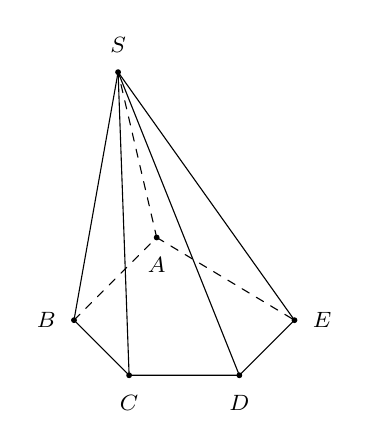
\begin{tikzpicture}[scale=0.7, font=\footnotesize, line join=round, line cap=round]
\foreach \x\y\t in {1.5/0/A,0/-1.5/B,1/-2.5/C,3/-2.5/D,4/-1.5/E,0.8/3/S}
\coordinate (\t) at (\x,\y);
\draw (S)--(B)--(C)--(D)--(E)--(S);
\draw [dashed] (B)--(A)--(S);
\draw[dashed] (A)--(E);
\draw (S)--(C) (S)--(D);
\foreach \t/\g in {A/-90,B/180,C/-90,D/-90,E/0,S/90} \draw[fill=black] (\t) circle(1.2pt) node[shift={(\g:10pt)}]{$\t$};
\end{tikzpicture} }}
\end{ex}

\begin{ex}%[1H4N4-1]%[Pj10-1-HK1-NH23-24-TeamTeXHoa-VUNgocHao]
Cho hình lập phương $ABCD.A' B' C' D'$. Chọn khẳng định đúng.
\choice
{\True $(ABCD) \parallel \left(A' B' D'\right)$}
{$\left(A' D' C\right) \parallel(A B C D)$}
{ $\left(D' C' A\right) \parallel(A B C D)$}
{$\left(B C C' B'\right) \parallel(A B C D)$}
\loigiai{
\begin{center}
\begin{tikzpicture}[scale=.7,font=\footnotesize, line join=round, line cap=round, >=stealth]
\tkzDefPoints{0/0/A,-1/-1.2/B,4/0/D}
\coordinate (C) at ($(B)+(D)-(A)$);
\coordinate (A') at ($(A)+(0,4)$);
\coordinate (B') at ($(A')+(B)-(A)$);
\coordinate (C') at ($(A')+(C)-(A)$);
\coordinate (D') at ($(A')+(D)-(A)$);
\draw (A')--(B')--(C')--(D')--(A')
(B)--(C)--(D)--(D')
(B)--(B')
(C)--(C') ;
\draw[dashed] (B)--(A)--(D)
(A)--(A') ;
\foreach \x/\g in {A/180,B/-120,C/-60,D/0,A'/120,B'/180,C'/100,D'/80} \fill[black](\x) circle (1pt) ($(\x)+(\g:4mm)$) node{$\x$};
\end{tikzpicture}
\end{center}
Theo định nghĩa hình lập phương ta được kết quả.
}
\end{ex}

\begin{ex}%[1D2H2-3]
Cho dãy số $\left(u_n\right)$ có số hạng tổng quát là $u_{n}=2\cdot3^n$ với $n\in\mathbb{N^*}$. Công thức truy hồi của dãy số đó là
\choice
{$\heva{&u_1=6\\&u_n=6u_{n-1},n>1}$}
{\True $\heva{&u_1=6\\&u_n=3u_{n-1},n>1}$}
{$\heva{&u_1=3\\&u_n=3u_{n-1},n>1}$}
{$\heva{&u_1=3\\&u_n=3u_{n-1},n>1}$}
\loigiai{ Ta có $u_1=2\cdot3^1=6$.\\  $u_{n-1}=2\cdot 3^{n-1}\Rightarrow3u_{n-1}=2\cdot 3^{n}=u_n$.}
\end{ex}

\begin{ex}%[1D1N3-1]
Mệnh đề nào dưới đây đúng với mọi $a$, $b$?
\choice
{$\cos{\left(a - b \right)} = \sin{a} \sin{b} - \cos{a}\cos{b}$}
{\True $\cos{\left(a - b \right)} = \cos{a}\cos{b} + \sin{a} \sin{b}$}
{$\cos{\left(a - b \right)} = \cos{a}\cos{b} - \sin{a} \sin{b}$}
{$\cos{\left(a - b \right)} = \cos{a}\sin{b} + \sin{a} \cos{b}$}
\loigiai{
Ta có $\cos{\left(a - b \right)} = \cos{a}\cos{b} + \sin{a} \sin{b}$.
}
\end{ex}

\begin{ex}%[1D5N1-2]%[Dự án đề kiểm tra Toán 11 GHKI NH23-24- Nguyễn Cường]%[THPT - Tp HCM]
Tuổi thọ (năm) của $50$ bình ác quy ô tô được cho như sau
\begin{center}
\begin{tabular}{|c|c|c|c|c|c|c|}
\hline
Tuổi thọ (năm)  & $[2;2{,}5)$ & $[2{,}5;3)$ & $[3;3{,}5)$ & $[3{,}5;4)$ & $[4;4{,}5)$ & $[4{,}5;5)$ \\
\hline
Tần số  & $4$ & $9$ & $14$ & $11$ & $7$ & $5$ \\
\hline
\end{tabular}
\end{center}
Cỡ mẫu của mẫu số liệu ghép nhóm trên là
\choice
{\True $50$}
{$48$}
{$14$}
{$6$}
\loigiai{
Cỡ mẫu của mẫu số liệu ghép nhóm trên là $n=4+9+14+11+7+5=50$.
}
\end{ex}

\begin{ex}%[1H4N6-1]
Phép chiếu song song biến ba đường thẳng song song thành
\choice
{ba đường thẳng đôi một song song với nhau}
{một đường thẳng}
{thành hai đường thẳng song song}
{\True cả ba trường hợp trên}
\loigiai{
Phép chiếu song song biến ba đường thẳng song song thành ba đường thẳng đôi một song song hoặc một đường thẳng hoặc thành hai đường thẳng song song.
}
\end{ex}

\begin{ex} %[1D2N3-1]
Trong các dãy số sau, dãy số nào không phải là một cấp số nhân?
\choice{$2;4;8;16;\ldots$}
{$1;-1;1;-1;\ldots$}
{\True $1^2;2^2;3^2; 4^2;\ldots$}
{$a;a^3;a^5;a^7;\ldots \; \left(a\ne 0\right)$}
\loigiai{
Dãy $1^2;2^2;3^2; 4^2;\cdots$ không phải là một cấp số nhân.
}
\end{ex}

\begin{ex}%[1D3N1-1]%[Dự án đề ôn tập Toán khối 11 NH23-24-Đợt 1- Bùi Thanh Cương]%[CTST-Đề số 08]
Cho hai dãy $\left(u_n\right)$ và $\left(v_n\right)$ thỏa mãn $\lim u_n=2$ và $\lim v_n=3.$ Giá trị của $\lim\left(u_n+v_n\right)$ bằng
\choice
{$ 6$}
{\True $ 5$}
{$-1$}
{$ 1$}
\loigiai{
Ta có $\lim\left(u_n+v_n\right)= \lim u_n+ \lim v_n=2+3=5$.
}

\end{ex}

\begin{ex}%[1D1N5-1]
Mệnh đề nào sau đây đúng với mọi $k$ là số nguyên
\choice
{\True $\cot{x} = \cot{\alpha} \Leftrightarrow x = \alpha + k \pi$}
{$\cot{x} = \cot{\alpha} \Leftrightarrow x = \pm \alpha + k \pi$}
{$\cot{x} = \cot{\alpha} \Leftrightarrow x = \pm \alpha + k2 \pi$}
{$\cot{x} = \cot{\alpha} \Leftrightarrow x = \pm \alpha + 2k$}
\loigiai{
Theo phương trình lượng giác cơ bản ta có $\cot{x} = \cot{\alpha} \Leftrightarrow x = \alpha + k \pi$ với $k \in \mathbb{Z}$.
}
\end{ex}

\begin{ex}%[1H4H2-2]%[Dự án đề ôn tập Toán Khối 11 HK1 NH23-24-Dot 1-Vương Quốc Phong]%[CTST - Đề số 3]
Trong không gian, cho hai đường thẳng $a$ và $b$ chéo nhau. Một đường thẳng $c$ song song với $a$. Khẳng định nào sau đây là đúng?
\choice
{$b$ và $c$ chéo nhau}
{$b$ và $c$ cắt nhau}
{\True $b$ và $c$ chéo nhau hoặc cắt nhau}
{$b$ và $c$ song song với nhau}
\loigiai{
Ta xét lần lượt các phương án
\begin{itemize}
\item \lq\lq $b$ và $c$ chéo nhau\rq\rq\ là sai vì $b$, $c$ có thể cắt nhau.
\item \lq\lq $b$ và $c$ cắt nhau\rq\rq\ là sai vì $b$, $c$ có thể chéo nhau.
\item \lq\lq $b$ và $c$ song song với nhau\rq\rq\ là sai vì nếu $b$ và $c$ song song thì $a$ và $b$ song song hoặc trùng nhau.
\end{itemize}
}
\end{ex}

\begin{ex}%[Pj10-Đề 07 HK1 NH2023-2024 CTST]%[Nguyễn Văn Nay]%[1D3N1-2]
Tìm giới hạn $\lim \dfrac{3n-1}{2n+1}$.
\choice
{$\dfrac{2}{3}$}
{$3$}
{$0$}
{\True $\dfrac{3}{2}$}
\loigiai{
Ta có $\lim \dfrac{3n-1}{2n+1}
=\lim \dfrac{3-\dfrac{1}{n}}{2+\dfrac{1}{n}}
=\dfrac{\lim \left(3-\dfrac{1}{n} \right)}{\lim \left(2+\dfrac{1}{n} \right)}
=\dfrac{\lim 3-\lim \dfrac{1}{n}}{\lim 2+\lim \dfrac{1}{n}}
=\dfrac{3-0}{2+0}=\dfrac{3}{2}$.
}
\end{ex}

\begin{ex}.%[1H4V1-3]
Cho tứ giác $A B C D$ và một điểm $S$ không thuộc mặt phẳng $(A B C D)$. Trên đoạn $S C$ lấy một điểm $M$ không trùng với $S$ và $C$. Gọi $N$ là giao điểm của đường thẳng $S D$ với mặt phẳng $(A B M)$. Khi đó $A N$ là giao tuyến của hai mặt phẳng nào sau đây?
\choice
{  $A N=(A B M) \cap(S B C)$}
{ $A N=(A B M) \cap(S C D)$}
{\True $A N=(A B M) \cap(S A D)$}
{ $A N=(A B M) \cap(S A C)$}
\loigiai{
\immini{Ta có $B \in(A B M) \cap(S B D).\quad(1)$\\
Gọi $O=A C \cap B D, K=A M \cap S O$. Khi đó\\
$
\heva{&K \in A M \subset(A B M) \\
&K \in S O \subset(S B D)} \Rightarrow K \in(A B M) \cap(S B D).\quad(2)    $\\
Từ (1) và $(2)$ suy ra $(A B M) \cap(S B D)=B K$.\\
Trong mặt phẳng $(S B D)$, gọi $N=B K \cap S D$. Khi đó\\
$
\heva{  &N \in S D \\
&N \in B K \subset(A B M)}
\Rightarrow N=(A B M) \cap S D .$\\
Dễ thấy $ A N=(A B M) \cap (S A D).$}
{\begin{tikzpicture}[>=stealth,line join=round, line cap=round, scale=1]
\coordinate[label=above left:$S$] (S) at (1,4) ;
\coordinate [label=below left:$B$](B) at (0,-0.5) ;
\coordinate [label=below left:$A$](A) at (-1,1) ;
\coordinate [label=below:$C$](C) at (3,-1.5) ;
\coordinate [label=right:$D$](D) at (5,1);
\coordinate[label=below  right:$M$](M) at ($(S)!1/3!(C)$);
\coordinate [label=below:$O$] (O) at (intersection of A--C and B--D);
\coordinate [label=below right:$K$] (K) at (intersection of A--M and S--O);
\coordinate [label=above right:$N$] (N) at (intersection of B--K and S--D);
%   \coordinate[label=above right:$N$] (N) at ($(S)!0.5!(D)$);
\draw (S)--(B)--(C)--(D)--cycle (B)--(A)--(S)--(C) ;
\draw[dashed] (B)--(D)--(A)--(C) (S)--(O) (A)--(M) (B)--(N)
;
\foreach \diem in {S,A,B,C,D, M, N,O,K} \fill (\diem)circle(1.5pt);
\end{tikzpicture}
}}

\end{ex}

\begin{ex}%[1D1H2-2]
Bảng giá trị nào dưới đây là bảng giá trị của hàm số $y=\cot x$ trên khoảng $(\pi{;}2 \pi)$
\choice
{   \begin{tabular}{|c|c|c|c|c|c|c|c|}
\hline
\raisebox{1cm}{\phantom{}}$x$ & $\dfrac{7 \pi}{6}$ & $\dfrac{5 \pi}{4}$ & $\dfrac{4 \pi}{3}$ & $\dfrac{3 \pi}{2}$ & $\dfrac{5 \pi}{3}$ & $\dfrac{7 \pi}{4}$ & $\dfrac{11 \pi}{6}$\\[0.5cm]
\hline
\raisebox{1cm}{\phantom{}}$\cot x$ & $\sqrt{3}$ & $1$ & $\dfrac{\sqrt{3}}{3}$ & $||$ & $-\dfrac{\sqrt{3}}{3}$ & $-1$ & $-\sqrt{3}$ \\[0.5cm]
\hline
\end{tabular}
}
{\True  \begin{tabular}{|c|c|c|c|c|c|c|c|}
\hline
\raisebox{1cm}{\phantom{}} $x$ & $\dfrac{7 \pi}{6}$ & $\dfrac{5 \pi}{4}$ & $\dfrac{4 \pi}{3}$ & $\dfrac{3 \pi}{2}$ & $\dfrac{5 \pi}{3}$ & $\dfrac{7 \pi}{4}$ & $\dfrac{11 \pi}{6}$ \\[0.5cm]
\hline
\raisebox{1cm}{\phantom{}} $\cot x$ & $\sqrt{3}$ & 1 & $\dfrac{\sqrt{3}}{3}$ & $0$ & $-\dfrac{\sqrt{3}}{3}$ & $-1$ & $-\sqrt{3}$ \\[0.5cm]
\hline
\end{tabular}
}
{   \begin{tabular}{|c|c|c|c|c|c|c|c|}
\hline
\raisebox{1cm}{\phantom{}} $x$ & $\dfrac{7 \pi}{6}$ & $\dfrac{5 \pi}{4}$ & $\dfrac{4 \pi}{3}$ & $\dfrac{3 \pi}{2}$ & $\dfrac{5 \pi}{3}$ & $\dfrac{7 \pi}{4}$ & $\dfrac{11 \pi}{6}$ \\[0.5cm]
\hline
\raisebox{1cm}{\phantom{}} $\cot x$ & $\sqrt{3}$ & $1$ & $\dfrac{\sqrt{3}}{3}$ & $\infty$ & $-\dfrac{\sqrt{3}}{3}$ & $-1$ & $-\sqrt{3}$ \\[0.5cm]
\hline
\end{tabular}
}
{   \begin{tabular}{|c|c|c|c|c|c|c|c|}
\hline
\raisebox{1cm}{\phantom{}} $x$ & $\dfrac{7 \pi}{6}$ & $\dfrac{5 \pi}{4}$ & $\dfrac{4 \pi}{3}$ & $\dfrac{3 \pi}{2}$ & $\dfrac{5 \pi}{3}$ & $\dfrac{7 \pi}{4}$ & $\dfrac{11 \pi}{6}$ \\[0.5cm]
\hline
\raisebox{1cm}{\phantom{}} $\cot x$ & $\sqrt{3}$ & 1 & $\dfrac{\sqrt{3}}{3}$ & không xác định & $-\dfrac{\sqrt{3}}{3}$ & $-1$ & $-\sqrt{3}$ \\[0.5cm]
\hline
\end{tabular}}
\loigiai{
Vì giá trị  $\cot\left(\dfrac{3 \pi}{2}\right)=0$ chứ không phải không xác định thể hiện ở các phương án khác.
}
\end{ex}

\begin{ex}%[1D5H1-3]%[Dự án đề ôn tập HKI Toán 11 NH23-24- Dương Phước Sang]%[CTST]
Khảo sát thời gian tập thể dục trong ngày của $1$ số học sinh khối $11$ thu được mẫu số liệu ghép nhóm sau:
\begin{longtable}{|c|c|c|c|c|c|}
\hline
Thời gian (phút) & $[0;20)$ & $[20;40)$ & $[40;60)$ & $[60;80)$ & $[80;100)$\\
\hline
Số học sinh & $5$ & $9$ & $12$ & $10$ & $6$\\
\hline
\end{longtable}
Hãy ước lượng thời gian tập thể dục trung bình của một học sinh trong một ngày.
\choice
{$53{,}41$}
{\True $51{,}43$}
{$38{,}02$}
{$42{,}83$}
\loigiai{
Bảng dữ liệu ghép nhóm có $\overline{x}=\dfrac{10\cdot 5+30\cdot 9+50\cdot 12+70\cdot 10+90\cdot 6}{5+9+12+10+6}=\dfrac{360}{7} \approx 51{,}43$.
}
\end{ex}

\begin{ex}%[1D2H1-3]
Cho dãy số $(u_n)$ có $u_1=-3$ và $u_{n+1}=u_n+n$ với $n\ge 1$, $n\in \mathbb{N}$. Số hạng thứ $3$ của dãy số đã cho là
\choice
{$u_3=-1$}
{$u_3=3$}
{$u_3=-2$}
{\True $u_3=0$}
\loigiai{
Ta có $u_1=-3$ và $u_{n+1}=u_n+n$ với $n\ge 1$, $n\in \mathbb{N}$.\\
Suy ra $u_2=u_1+1=-3+1=-2$; $u_3=u_2+2=-2+2=0$.
}
\end{ex}

\begin{ex}%[1D3N2-1]%[Dự án đề kiểm tra Toán 11 HHKI NH23-24- Phạm Văn Long]%[Thi thử - KNTT]
Cho hai hàm số $f\left(x\right),g\left(x\right)$ thỏa mãn ${\mathop{\lim}\limits_{x\to 2}} f\left(x\right)=5$ và ${\mathop{\lim}\limits_{x\to 2}} g\left(x\right)=1$. Giá trị của ${\mathop{\lim}\limits_{x\to 2}} \left[f\left(x\right)\cdot g\left(x\right)\right]$ bằng
\choice{\True $5$}
{$6$}
{$1$}
{$-1$}
\loigiai{
Ta có ${\mathop{\lim}\limits_{x\to 2}} \left[f\left(x\right)\cdot g\left(x\right)\right]={\mathop{\lim}\limits_{x\to 2}} f\left(x\right)\cdot {\mathop{\lim}\limits_{x\to 2}} g\left(x\right)=5\cdot 1=5$.
}
\end{ex}

\begin{ex}%[Dự án TeX GKI 11, Đoàn Hùng]%[1D2H2-6]
Tìm tổng $S$ của $100$ số nguyên dương đầu tiên và đều chia $5$ dư $1$.
\choice
{\True $24850$ }
{ $25100$ }
{ $50200$ }
{ $5001$ }
\loigiai{
Các số chia $5$ dư $1$ tạo thành cấp số cộng có $u_1=1$ và $d=5$, do đó
\[S_{100}=\dfrac{100\cdot (2u_1+99d)}{2}=\dfrac{100\cdot (2\cdot 1+99\cdot 5)}{2}=24850.\]
}
\end{ex}

\begin{ex}%[1H4H6-2]%[Dự án đề kiểm tra Toán 11 HKI NH23-24-Đợt 1- Phạm Phương]%[CTST-Đề số 5]
%[TH]
Cho tam giác $ABC$ ở trong mặt phẳng $\left(\alpha \right)$ và phương $l$. Biết hình chiếu theo phương $l$ của tam giác $ABC$ lên mặt phẳng $\left(P\right)$ là một đoạn thẳng. Khẳng định nào sau đây đúng?
\choice
{$\left(\alpha \right)\parallel \left(P\right)$}
{$\left(\alpha \right)\equiv \left(P\right)$}
{\True $l \parallel \left(\alpha \right)$ hoặc $l \subset \left(\alpha \right)$}
{$l\subset \left(\alpha \right)$}
\loigiai{
Vì hình chiếu theo phương $l$ của tam giác $ABC$ lên mặt phẳng $\left(P\right)$ là một đoạn thẳng nên $l \parallel \left(\alpha \right)$ hoặc $l\subset \left(\alpha \right)$.
}
\end{ex}

\begin{ex}%[1D3V3-3]
Cho hàm số $f(x) =\heva{&\dfrac{\sqrt{2x^2 -3x +5}-2}{1-x}\quad \text{khi} \,\, x\ne 1\\& m +2 \, \text{khi}\, x =1}.$ Hàm số liên tục tại điểm $x=1$ khi $m=-\dfrac{a}{b}$ với $\dfrac{a}{b}$ tối giản, $a,b\in\mathbb{N}$. Khi đó, tổng $a + b$ bằng:
\choice
{\True $13$}
{$5$}
{$3$}
{$6$}
\loigiai{
Tập xác định $\mathrm{D}=\mathbb{R}$.\\
Ta có: $f(1) = m + 2$
\begin{align*}
\displaystyle\lim_{x\to 1}f(x) & = \displaystyle\lim_{x\to 1}\dfrac{\sqrt{2x^2 -3x +5}-2}{1-x} = \displaystyle\lim_{x\to 1}\dfrac{2x^2 -3x +5 -4}{(1-x)\left(\sqrt{2x^2 -3x +5}+2\right)}\\
&=\displaystyle\lim_{x\to 1}\dfrac{2x^2 - 3x +1}{(1-x)\left(\sqrt{2x^2 -3x +5}+2\right)}=\displaystyle\lim_{x\to 1}\dfrac{(x-1)(2x -1)}{(1-x)\left(\sqrt{2x^2 -3x +5}+2\right)}\\
& =\displaystyle\lim_{x\to 1}\dfrac{2x-1}{-\left(\sqrt{2x^2 -3x +5}+2\right)}
= -\dfrac{1}{4}.
\end{align*}
Hàm số liên tục tại điểm $x=1 \Leftrightarrow \displaystyle\lim_{x\to 1}f(x) = f(1)$ $\Leftrightarrow m +2 = -\dfrac{1}{4} \Leftrightarrow m =-\dfrac{9}{4}$.\\
Vì $m=-\dfrac{a}{b}$ nên $\heva{&a = 9\\& b=4}$. Vậy $a + b = 13$.
}
\end{ex}

\begin{ex}%[1H4H3-2]
Cho hình chóp $S.ABCD$ có đáy $ABCD$ là hình bình hành. Gọi $G_1,G_2$, lần lượt là trọng tâm các tam giác $SAB$, $SCD$. Xét các khẳng định sau:
\begin{enumEX}[(I)]{2}
\item $G_1G_2\parallel (SBC)$.
\item $G_1G_2\parallel (SAD)$.
\item \,$G_1G_2\parallel (SAC)$.
\item \,$G_1G_2\parallel (ABD)$.
\end{enumEX}
Các khẳng định đúng là
\choice
{\True (I), (II), (IV)}
{(I), (II), (III)}
{(I), (IV)}
{(III), (IV)}
\loigiai{
\begin{center}
\begin{tikzpicture}[scale=1,font=\footnotesize,line join=round,line cap=round,>=stealth]
\def\a{4}
\path   (0:0) coordinate (A)
++(0:\a) coordinate (D)
++(-150:\a/2) coordinate (C)
($(A)+(C)-(D)$) coordinate (B)
($(A)+(80:\a)$) coordinate (S)
($(B)!0.5!(A)$) coordinate (M)
($(C)!0.5!(D)$) coordinate (N)
($(S)!2/3!(N)$) coordinate (G_2)
($(S)!2/3!(M)$) coordinate (G_1)
;
\draw[dashed,thick]     (B)--(A)--(D)   (A)--(S)--(M)--(N) (G_1)--(G_2);
\draw[thick]            (B)-- (C)--(D) (S)--(N)
(B)--(S)    (C)--(S)    (D)--(S);
\foreach \x/\g in {A/-45,B/-135,C/-45,D/45,S/90,N/-45,G_2/0,M/-45,G_1/-45}
\fill[black]    (\x) circle (1pt)
($(\g:3mm)+(\x)$) node {$\x$};
\end{tikzpicture}
\end{center}
Gọi $M, N$ lần lượt là trung điểm của $AB, CD$.\\
Do $G_1,G_2$ lần lượt là trọng tâm $\triangle SAB$ và $\triangle SCD$ nên $\dfrac{SG_1}{SM}=\dfrac{SG_2}{SN}=\dfrac{2}{3}\Rightarrow G_1G_2\parallel MN$.\\
Mà $MN\subset (ABCD)$ suy ra $G_1G_2\parallel (ABCD)$.\\
Ta có $MN\parallel AD\parallel BC\Rightarrow G_1G_2\parallel AD\parallel BC$.\\
Mà $BC\subset (SBC)$ và $AD\subset (SAD)$, suy ra $G_1G_2\parallel (SAD)$, $G_1G_2\parallel (SBC)$.
}
\end{ex}

\begin{ex}%[1H4H1-4]
%\immini{
Cho hình chóp $S.ABCD$ có đáy $ABCD$ là hình bình hành tâm $O$. Gọi $M$, $N$, $K$ lần lượt là trung điểm của $CD$, $CB$, $SA$. Gọi $H$ là giao điểm của $AC$ và $MN$. Giao điểm của $SO$ với $(MNK)$ là điểm $E$. Khi đó
\choice
{$E$ là giao của $M N$ với $SO$}
{$E$ là giao của $K N$ với $SO$.}
{\True $E$ là giao của $K H$ với $SO$}
{$E$ là giao của $K M$ với $SO$}
\loigiai{
\immini{        Trong mặt phẳng $(SAC)$, gọi $E=KH \cap SO$.\\
Khi đó $\heva{&E \in KH \subset (KMN)\\ &E \in SO} \Rightarrow E=SO \cap (KMN)$.}
{        \begin{tikzpicture}[scale=0.8, font=\footnotesize,line join=round, line cap=round, >=stealth]
\coordinate (A) at (0,0);
\coordinate (B) at (-2,-2);
\coordinate (D) at (5,0);
\coordinate (C) at ($(B)+(D)-(A)$);
\coordinate (O) at ($(A)!0.5!(C)$);
\coordinate (S) at ($(O)+(0,5)$);
\coordinate (M) at ($(C)!0.5!(B)$);
\coordinate (N) at ($(D)!0.5!(C)$);
\coordinate (K) at ($(S)!0.5!(A)$);
\coordinate (H) at ($(M)!0.5!(N)$);
\coordinate (E) at (intersection of K--H and S--O);
\\foreach \\i in {A,B,C,D}{\\draw (S)--(\\i);}
\\draw (B)--(C)--(D);
\\draw[dashed,thin](S)--(A)--(B)--(D)--(A)--(C);
\draw(S)--(B) (S)--(C) (N)--(S)--(D) (B)--(C)--(D);
\draw[dashed,thin](S)--(A)--(C)--(M) (A)--(B) (A)--(D)--(B) (S)--(O) (A)--(N)--(M)--(K)--(N) (K)--(H);
\foreach \i/\g in {S/90,A/-90,B/-90,C/-90,D/-90,O/-90,M/-90,N/0,K/-150,H/-90,E/180}{\draw[fill=black](\i) circle (1.5pt) ($(\i)+(\g:4mm)$) node[scale=1]{$\i$};}
\end{tikzpicture}}
}
\end{ex}

\begin{ex}%[Pj10-1-GK1-NH23-24--TeamTeXHoa--Lâm Chính]%[1D2N1-4]
Dãy số nào sau đây là dãy số tăng?
\choice
{\True $-1$, $1$, $3$, $5$, $7$}
{$1$, $4$, $16$, $9$, $25$}
{$0$, $3$, $8$, $24$, $15$}
{$0$, $3$, $12$, $9$, $6$}
\loigiai{
Ta thấy $-1 < 1 < 3 < 5 < 7$ nên dãy số $-1$, $1$, $3$, $5$, $7$ là dãy số tăng.
}
\end{ex}


\noindent\textbf{II. PHẦN TỰ LUẬN:}
\begin{ex}%[1D1H5-3]%[Dự án đề kiểm tra Toán 11 GHKI NH23-24- Võ Thị Thùy Trang]%[THPT Võ Thị Sáu - Tp HCM]
Giải phương trình sau $\sin 2x-5\cos x=0$.
\loigiai{
Ta có
\allowdisplaybreaks
\begin{eqnarray*}
&&\sin 2x-5\cos x=0\\
&\Leftrightarrow& 2\sin x\cdot\cos x-5\cos x=0\\
&\Leftrightarrow& \cos x\left(2\sin x-5\right)=0\\
&\Leftrightarrow&\hoac{&\cos x=0\\&\sin x=\dfrac{5}{2}\notin[-1;1]}\\
&\Leftrightarrow& x=\dfrac{\pi}{2}+k\pi,\,(k\in {\mathbb{Z}}).
\end{eqnarray*}
}

\end{ex}

\begin{ex}%[Pj08-0-GK1-NH23-24--TeamTeXHoa--LeQuan]%[1D3V2-5]
Tính giới hạn  $\lim\limits_{x\to -\infty} \left(\sqrt{x^2-4x}-\sqrt{x^2-x}\right)$
\loigiai{
Ta có
\begin{eqnarray*}
&&\lim\limits_{x\to -\infty} \left(\sqrt{x^2-4x}-\sqrt{x^2-x}\right)\\
&=& \lim\limits_{x\to -\infty} \dfrac{(x^2-4x)-(x^2-x)}{\sqrt{x^2-4x}+\sqrt{x^2-x}}\\
&=& \lim\limits_{x\to -\infty} \dfrac{-3x}{-x\left(\sqrt{1-\frac{4}{x}}+\sqrt{1-\frac{1}{x}}\right)}\\
&=& \dfrac{3}{2}.
\end{eqnarray*}

}\end{ex}

\begin{ex}%[1D3T1-5]
Cho tam giác đều $A_1B_1C_1$ cạnh $a$. Người ta dựng tam giác đều $A_2B_2C_2$ cạnh bằng đường cao của tam giác $A_1B_1C_1$. Dựng tam giác đều $A_3B_3C_3$ cạnh bằng đường cao của tam giác $A_2B_2C_2$ và cứ tiếp tục như vậy. Tính tổng diện tích $S$ của tất cả các tam giác đều $A_1B_1C_1$, $A_2B_2C_2$, $A_3B_3C_3$, \ldots.
\loigiai{
Tam giác $A_1B_1C_1$ có diện tích $S_1=\dfrac{a^2\sqrt{3}}{4}$.\\
Tam giác $A_2B_2C_2$ có cạnh là $a_2=\dfrac{a\sqrt{3}}{2}$ nên $A_2B_2C_2$ có diện tích $S_2=\dfrac{3}{4}\cdot\dfrac{a^2\sqrt{3}}{4}=\dfrac{3}{4}S_1$.\\
Tam giác $A_3B_3C_3$ có cạnh là $a_3=\dfrac{a_2\sqrt{3}}{2}$ nên $A_3B_3C_3$ có diện tích $S_3=\dfrac{3}{4}\cdot\dfrac{a_2^2\sqrt{3}}{4}=\dfrac{3}{4}S_2=\left(\dfrac{3}{4}\right)^2S_1.$\\
...\\
Vậy diện tích các tam giác tạo thành là một cấp số nhân với công bội $q=\dfrac{3}{4}$.\\
Suy ra tổng diện tích tất cả các tam giác là $S=\dfrac{S_1}{1-q}=\dfrac{\dfrac{a^2\sqrt{3}}{4}}{1-\dfrac{3}{4}}=a^2\sqrt{3}$.}
\end{ex}

\begin{ex} %[1H4C4-6]
Cho hình chóp $S.ABCD$ có đáy là hình thang $ABCD$, $AB\parallel CD$, $AB=2CD$, tam giác $SAB$ đều cạnh $2a$, $M$ là điểm thuộc cạnh $AD$ sao cho $MD=2MA$, $( \alpha )$ là mặt phẳng qua $M$ song song với mặt phẳng $( SAB )$ cắt các cạnh $BC$, $SC$, $SD$ lần lượt tại $N$, $P$, $Q$. Tính diện tích tứ giác $MNPQ$.

\loigiai{
\immini{Ta có $\heva{
& ( \alpha )\parallel( SAB ) \\
& ( ABCD )\cap ( SAB )=AB \\
& M\in ( \alpha )\cap ( ABCD ) \\
}\\\Rightarrow ( \alpha )\cap ( ABCD )=d_1,$ $d_1$ đi qua $M$ và song song với $AB$, cắt $BC$ tại $N$.\\
Tương tự $( \alpha )\cap ( SBC )=d_2$, $d_2$ đi qua $N$ và song song với $SB$, cắt $SC$ tại $P$,\\
$( \alpha )\cap ( SCD )=d_3$, $d_3$ đi qua $P$ và song song với $CD$ và $AB$, cắt $SD$ tại $Q$.\\
Ta có $\heva{
& ( \alpha )\parallel( SAB ) \\
& ( SAB )\cap ( SAD )=SA \\
& ( \alpha )\cap ( SAD )=QM \\
}\Rightarrow QM\parallel SA.$\\}
{\begin{tikzpicture}[scale=0.6, font=\footnotesize, line join=round, line cap=round, >=stealth]
\def\bc{4} % cạnh AD
\def\ba{3.5} % cạnh BA
\def\h{5} % đường cao
\def\gocB{40} % góc B của đáy
\coordinate[label=below left:$D$] (D) at (0,0);
\coordinate[label=above right:$A$] (A) at (\gocB:\ba);
\coordinate[label=below:$C$] (C) at (\bc,0);
\coordinate (I) at ($(A)+(0:\bc)$);
\coordinate[label=right:$B$] (B) at ($(A)!2!(I)$);
\coordinate[label=above:$S$] (S) at ($(A)+(80:\h)$);
\coordinate[label= left:$M$] (M) at ($(A)!1/3!(D)$);
\coordinate[label= below right:$N$] (N) at ($(B)!1/3!(C)$);
\coordinate[label= left:$Q$] (Q) at ($(S)!1/3!(D)$);
\coordinate[label= right:$P$] (P) at ($(S)!1/3!(C)$);
\draw (B)--(C)--(D)--(S)--cycle (S)--(C) (Q)--(P)--(N);
\draw[dashed] (A)--(D) (S)--(A)--(B) (Q)--(M)--(N);
\foreach \diem in {A,B,C,D,S,Q,P,M,N}   \fill (\diem)circle(1.5pt);
\end{tikzpicture}}
Trong hình thang $ABCD$, ta có $MN=\dfrac{1}{3}CD+\dfrac{2}{3}AB=\dfrac{5a}{3}$.\\
Xét $\Delta SAD$ có $QM\parallel SA\Rightarrow \dfrac{QM}{SA}=\dfrac{DM}{DA}=\dfrac{2}{3}\Rightarrow QM=\dfrac{4a}{3}.$\\
Xét $\Delta SCD$ có $PQ\parallel CD\Rightarrow \dfrac{PQ}{CD}=\dfrac{SQ}{SD}=\dfrac{AM}{AD}=\dfrac{1}{3}\Rightarrow PQ=\dfrac{a}{3}$.\\
Xét $\Delta SBC$ có $PN\parallel SB\Rightarrow \dfrac{PN}{SB}=\dfrac{CP}{CS}=\dfrac{2}{3}\Rightarrow PN=\dfrac{4a}{3}$.\\
\immini{Trong hình thang cân $MNPQ$, kẻ $QH\perp MN,PF\perp MN$.\\
Ta có $HF=PQ=\dfrac{a}{3},MH=FN=\dfrac{\dfrac{5a}{3}-\dfrac{a}{3}}{2}=\dfrac{2a}{3}$, $QH=\sqrt{M{{Q}^2}-M{{H}^2}}=\sqrt{\dfrac{16a^2}{9}-{{\dfrac{4a}{9}}^2}}=\dfrac{2a\sqrt{3}}{3}$.}
{\begin{tikzpicture}[scale=0.8, font=\footnotesize, line join=round, line cap=round, >=stealth]
\def\b{4}
\def\r{3}
\def\goc{30}
\coordinate (M) at (0,0);
\coordinate (Q) at (\goc:\r);
\coordinate (P) at ($(Q)+(0:\b/2)$);
\coordinate (N) at ($(P)+(-\goc:\r)$);
\coordinate (H) at ($(Q)+(-90:\r/2)$);
\coordinate (F) at ($(P)+(-90:\r/2)$);
\draw (M)--(Q)--(P)--(N)--cycle (Q)--(H) (P)--(F);
\foreach \p/\i in {M/180,N/0,P/90,Q/90,H/-90,F/-90}
\fill (\p) circle (1.5pt) node[shift={(\i:3mm)}]{$\p$};
\end{tikzpicture}}
Diện tích hình thang $MNPQ$ là $\dfrac{\left(  \dfrac{a}{3}+\dfrac{5a}{3} \right) \cdot \dfrac{2a\sqrt{3}}{3}}{2}=\dfrac{2a^2\sqrt{3}}{3}$.
} \end{ex}
\Closesolutionfile{ans}
